% Seminar: Ipoteza Pieței Eficiente (EMH)
% Statistica Piețelor Financiare --- quantlets Colab

\documentclass[9pt, aspectratio=169, t]{beamer}
%=============================================================================
% PREAMBUL COMUN - Statistica Piețelor Financiare
% Versiune robustă pentru macOS (MacTeX / BasicTeX / TeX Live)
% Daniel Traian Pele, Antoaneta Amza - ASE București
%
% MODIFICĂRI față de varianta originală:
%  (1) fontawesome5 făcut OPȚIONAL (\IfFileExists) → nu mai pică dacă lipsește
%  (2) polyglossia cu fallback automat pe babel dacă romanian nu există
%  (3) setmainfont rescris cu Ligatures=TeX și nume normalizate (merge pe macOS)
%  (4) graphicspath extins (include directorul curent + variante relative) ca
%      logo-urile să fie găsite și când lansezi xelatex dintr-un subdirector
%
% Compilare:  xelatex preamble + main, de DOUĂ ori (toc/ref).
%=============================================================================

% Asigură încadrarea conținutului pe diapozitive
\setbeamersize{text margin left=8mm, text margin right=8mm}

%=============================================================================
% CONFIGURARE TEMĂ ȘI STIL
%=============================================================================
\usetheme{default}

% Paletă de Culori
\definecolor{MainBlue}{RGB}{26, 58, 110}
\definecolor{AccentBlue}{RGB}{26, 58, 110}
\definecolor{IDAred}{RGB}{205, 0, 0}
\definecolor{DarkGray}{RGB}{51, 51, 51}
\definecolor{MediumGray}{RGB}{128, 128, 128}
\definecolor{LightGray}{RGB}{248, 248, 248}
\definecolor{VeryLightGray}{RGB}{235, 235, 235}
\definecolor{KeynoteGray}{RGB}{218, 218, 218}
\definecolor{SectionGray}{RGB}{120, 120, 120}
\definecolor{FooterGray}{RGB}{100, 100, 100}
\definecolor{Crimson}{RGB}{220, 53, 69}
\definecolor{Forest}{RGB}{46, 125, 50}
\definecolor{Amber}{RGB}{181, 133, 63}
\definecolor{Orange}{RGB}{230, 126, 34}
\definecolor{Purple}{RGB}{142, 68, 173}

% Fundal gradient (gradient Keynote exact 315°: alb la RGB 218,218,218)
\setbeamertemplate{background}{%
	\begin{tikzpicture}[remember picture, overlay]
		\shade[shading=axis, shading angle=315,
		top color=white, bottom color=KeynoteGray]
		(current page.south west) rectangle (current page.north east);
	\end{tikzpicture}%
}
% Culoare solidă de rezervă pentru compatibilitate
\setbeamercolor{background canvas}{bg=}

\setbeamercolor{palette primary}{bg=MainBlue, fg=white}
\setbeamercolor{palette secondary}{bg=MainBlue!85, fg=white}
\setbeamercolor{palette tertiary}{bg=MainBlue!70, fg=white}
\setbeamercolor{structure}{fg=MainBlue}
\setbeamercolor{title}{fg=IDAred}
\setbeamercolor{frametitle}{fg=IDAred, bg=}
\setbeamercolor{block title}{bg=MainBlue, fg=white}
\setbeamercolor{block body}{bg=VeryLightGray, fg=DarkGray}
\setbeamercolor{block title alerted}{bg=Crimson, fg=white}
\setbeamercolor{block body alerted}{bg=Crimson!8, fg=DarkGray}
\setbeamercolor{block title example}{bg=Forest, fg=white}
\setbeamercolor{block body example}{bg=Forest!8, fg=DarkGray}
\setbeamercolor{item}{fg=MainBlue}

\setbeamerfont{institute}{size=\footnotesize}

\setbeamercolor{author in head/foot}{fg=FooterGray, bg=}
\setbeamercolor{title in head/foot}{fg=FooterGray, bg=}
\setbeamercolor{date in head/foot}{fg=FooterGray, bg=}
\setbeamercolor{section in head/foot}{fg=FooterGray, bg=}
\setbeamercolor{subsection in head/foot}{fg=FooterGray, bg=}

\setbeamertemplate{itemize item}{\color{MainBlue}$\boxdot$}
\setbeamertemplate{itemize subitem}{\color{MainBlue}$\blacktriangleright$}
\setbeamertemplate{itemize subsubitem}{\color{MainBlue}\tiny$\bullet$}
\setbeamertemplate{itemize/enumerate body begin}{\normalsize}
\setbeamertemplate{itemize/enumerate subbody begin}{\normalsize}

\setbeamertemplate{section in toc}{%
	\leavevmode\leftskip=1.5em%
	\llap{\color{MainBlue}$\boxdot$\kern0.5em}%
	\inserttocsection\par%
}

\setlength{\leftmargini}{10pt}
\setlength{\leftmarginii}{10pt}
\makeatletter
\def\@listi{\leftmargin\leftmargini \topsep 0pt \parsep 0pt \itemsep 0pt}
\def\@listii{\leftmargin\leftmarginii \topsep 0pt \parsep 0pt \itemsep 0pt}
\makeatother

\setbeamertemplate{navigation symbols}{}

%=============================================================================
% ANTET PERSONALIZAT
%=============================================================================
\setbeamertemplate{headline}{%
	\vskip10pt%
	\hbox to \paperwidth{%
		\hskip0.5cm%
		{\small\color{FooterGray}\renewcommand{\hyperlink}[2]{##2}\insertsectionhead}%
		\hfill%
		\textcolor{FooterGray}{\small\insertframenumber}%
		\hskip0.5cm%
	}%
	\vskip4pt%
	{\color{FooterGray}\hrule height 0.4pt}%
}

%=============================================================================
% PACHETE — ordine importantă: fontspec ÎNAINTE de polyglossia/babel
%=============================================================================

% --- (1) FONTSPEC + FONTURI ROBUSTE PE macOS ---
\usepackage{fontspec}
% Pe macOS unele fonturi Latin Modern nu sunt înregistrate ca fonturi de sistem.
% Folosim Ligatures=TeX (pentru -- → en-dash etc.) și lăsăm fontspec să caute
% prin kpathsea (merge atât pe Mac, cât și pe Linux/Windows).
\defaultfontfeatures{Ligatures=TeX}
\IfFontExistsTF{Latin Modern Roman}{%
	\setmainfont{Latin Modern Roman}
	\setsansfont{Latin Modern Sans}
	\setmonofont{Latin Modern Mono}
}{%
	% Fallback dacă numele cu spații nu sunt găsite (cazul macOS fără fonturi
	% Latin Modern în /Library/Fonts) — fontspec va folosi fontul implicit.
	\PackageWarning{preamble}{Latin Modern Roman nu a fost gasit; folosesc fontul implicit.}
}

% --- (2) POLYGLOSSIA SAU BABEL CU FALLBACK ---
% Pe versiuni vechi de polyglossia (TeX Live < 2020) limba `romanian` nu există.
% Detectăm și folosim babel ca rezervă.
\IfFileExists{gloss-romanian.ldf}{%
	\usepackage{polyglossia}
	\setdefaultlanguage{romanian}
	\setotherlanguage{english}
}{%
	\PackageWarning{preamble}{polyglossia/romanian indisponibil; folosesc babel.}
	\usepackage[english,romanian]{babel}
}

% --- (3) MATH ȘI GRAFICĂ ---
\usepackage{amsmath, amssymb, amsthm}
\usepackage{mathtools}
\usepackage{bm}
\usepackage{tikz}
\usetikzlibrary{arrows.meta, positioning, shapes, calc, decorations.pathreplacing, shadings}
\usepackage{booktabs}
\usepackage{multirow}
\usepackage{array}
\usepackage{graphicx}
\usepackage{hyperref}
\usepackage{colortbl}
\usepackage{listings}
\lstset{basicstyle=\ttfamily\small, breaklines=true, frame=single, backgroundcolor=\color{VeryLightGray}}
\hypersetup{colorlinks=true, linkcolor=MainBlue, urlcolor=MainBlue}

% --- (4) GRAPHICSPATH cu directorul curent inclus ca fallback ---
\graphicspath{{./}{./logos/}{./charts/}{./photos/}{../logos/}{../charts/}{../photos/}{../../logos/}{../../charts/}{../../photos/}}
\hfuzz=2pt
\vfuzz=2pt

%=============================================================================
% SUBSOL PERSONALIZAT — fontawesome5 făcut OPȚIONAL
%=============================================================================
% Pe BasicTeX / instalări minime de MacTeX, fontawesome5 nu există.
% Dacă lipsește, omitem icoanele (subsolul rămâne curat).
\IfFileExists{fontawesome5.sty}{%
	\usepackage{fontawesome5}
	\newcommand{\hasfontawesome}{true}
}{%
	\PackageWarning{preamble}{fontawesome5 indisponibil; subsolul nu va contine icoane.}
}

\setbeamertemplate{footline}{%
	{\color{FooterGray}\hrule height 0.4pt}%
	\vskip4pt%
	\hbox to \paperwidth{%
		\hskip0.5cm%
		\textcolor{FooterGray}{\small Statistica Piețelor Financiare}%
		\hfill%
		\raisebox{-0.1em}{%
			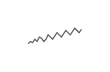
\begin{tikzpicture}[x=0.08em, y=0.08em, line width=0.4pt]
				\draw[FooterGray] (0,3) -- (1,4) -- (2,3.5) -- (3,5) -- (4,4) -- (5,6) -- (6,5.5) -- (7,4) -- (8,5) -- (9,7) -- (10,6) -- (11,5) -- (12,6.5) -- (13,8) -- (14,7) -- (15,6) -- (16,7.5) -- (17,9) -- (18,8) -- (19,7) -- (20,8.5) -- (21,10) -- (22,9) -- (23,8) -- (24,9.5);
			\end{tikzpicture}%
		}%
		\hskip0.5cm%
	}%
	\vskip6pt%
}

%=============================================================================
% COMANDA QUANTLET
%=============================================================================
\newcommand{\quantlet}[2]{%
	\hfill\href{#2}{%
		\raisebox{-0.15em}{
\includegraphics[height=0.7em]{ql_logo.png}}%
		\textcolor{MainBlue}{\tiny\ #1}%
	}%
}

%=============================================================================
% PAGINĂ TITLU PERSONALIZATĂ
%=============================================================================
\defbeamertemplate*{title page}{hybrid}[1][]
{
	\vspace{0.2cm}
	\noindent\makebox[\linewidth][s]{%
		\href{https://www.ase.ro}{
\includegraphics[height=1.0cm]{ase_logo.png}}\hfill%
		\href{https://theida.net}{
\includegraphics[height=1.0cm]{ida_logo.png}}\hfill%
		\href{https://blockchain-research-center.com}{
\includegraphics[height=1.0cm]{brc_logo.png}}\hfill%
		\href{https://www.ai4efin.ase.ro}{
\includegraphics[height=1.0cm]{ai4efin_logo.png}}\hfill%
		\href{https://ipe.ro/new}{
\includegraphics[height=1.0cm]{acad_logo.png}}\hfill%
		\href{https://www.digital-finance-msca.com}{
\includegraphics[height=1.0cm]{msca_logo.png}}%
	}
	\vspace{0.6cm}
	
	\noindent\makebox[\linewidth][c]{%
		\begin{minipage}{0.11\linewidth}
			\centering
			\href{https://quantlet.com}{
\includegraphics[height=1.1cm]{ql_logo.png}}
		\end{minipage}%
		\begin{minipage}{0.76\linewidth}
			\centering
			{\LARGE\bfseries\usebeamercolor[fg]{title}\inserttitle}
			
			\vspace{0.3cm}
			
			{\usebeamerfont{subtitle}\usebeamercolor[fg]{title}\insertsubtitle}
		\end{minipage}%
		\begin{minipage}{0.11\linewidth}
			\centering
			\href{https://quantinar.com}{
\includegraphics[height=1.1cm]{qr_logo.png}}
		\end{minipage}%
	}
	
	\vspace{0.6cm}
	
	\hspace{0.5cm}{\usebeamerfont{author}\insertauthor}
	
	\vspace{0.3cm}
	
	\hspace{0.5cm}\begin{minipage}[t]{0.9\textwidth}
		\raggedright\small\insertinstitute
	\end{minipage}
}
\setbeamertemplate{title page}[hybrid]

%=============================================================================
% MEDII PENTRU TEOREME
%=============================================================================
\theoremstyle{definition}
\setbeamertemplate{theorems}[numbered]
\newtheorem{defn}{Definiție}
\newtheorem{thm}{Teoremă}
\newtheorem{prop}{Propoziție}
\newtheorem{rmk}{Observație}

%=============================================================================
% CENTRED MINIPAGE
%=============================================================================
\newenvironment{cminipage}[1]{%
	\par\noindent\hfill\begin{minipage}{#1}\ignorespaces
	}{%
	\end{minipage}\hfill\null\par
}

%=============================================================================
% COMENZI PERSONALIZATE
%=============================================================================
\newcommand{\E}{\mathbb{E}}
\newcommand{\Var}{\text{Var}}
\newcommand{\Cov}{\text{Cov}}
\newcommand{\Corr}{\text{Corr}}
\newcommand{\VaR}{\text{VaR}}
\newcommand{\ES}{\text{ES}}
\newcommand{\R}{\mathbb{R}}
\newcommand{\N}{\mathbb{N}}
\newcommand{\Z}{\mathbb{Z}}
\newcommand{\B}{\mathbf{B}}
\newcommand{\imark}{\textcolor{MainBlue}{\textbullet}}
\newcommand{\RMSE}{\text{RMSE}}
\newcommand{\MAE}{\text{MAE}}
\newcommand{\MAPE}{\text{MAPE}}
\newcommand{\correct}{\textcolor{Forest}{\checkmark}}
\newcommand{\incorrect}{\textcolor{Crimson}{\texttimes}}

%=============================================================================
% INFORMAȚII TITLU
%=============================================================================
\title[Statistica Piețelor Financiare]{Statistica Piețelor Financiare}
\author[D.T. Pele, A. Amza]{\texorpdfstring{\begin{tabular}[t]{@{}l@{}}Daniel Traian PELE \\ Antoaneta Amza\end{tabular}}{Daniel Traian PELE, Antoaneta Amza}}
\institute{Academia de Studii Economice din București\\
	IDA Institute Digital Assets\\
	Blockchain Research Center\\
	AI4EFin Artificial Intelligence for Energy Finance\\
	Academia Română, Institutul de Prognoză Economică\\
	MSCA Digital Finance}
\date{}
\subtitle{Seminar EMH --- Ipoteza Pieței Eficiente (Efficient Market Hypothesis)}

\begin{document}

%=============================================================================
% PAGINA DE TITLU
%=============================================================================
{
\setbeamertemplate{headline}{}
\setbeamertemplate{footline}{}
\begin{frame}
    \titlepage
\end{frame}
}

% Colab base URL
\newcommand{\ch}[1]{\href{https://colab.research.google.com/github/QuantLet/Stat_fin_markets/blob/master/Ch_04/SFM_ch4_#1/SFM_ch4_#1.ipynb}{#1}}

%=============================================================================
% CUPRINS
%=============================================================================
\begin{frame}[shrink=15]{Cuprins (Contents)}
\begin{cminipage}{0.95\textwidth}
\begin{itemize}\setlength{\itemsep}{0pt}
    \item Partea I: Teorie EMH
    \begin{itemize}\setlength{\itemsep}{0pt}
        \item Cele 3 forme (Fama, 1970), random walk, martingal
    \end{itemize}
    \item Partea II: Testul de autocorelație (ACF + Ljung--Box)
    \begin{itemize}\setlength{\itemsep}{0pt}
        \item Exercițiu pe S\&P 500 (quantlet Colab)
    \end{itemize}
    \item Partea III: Variance ratio multi-piață
    \begin{itemize}\setlength{\itemsep}{0pt}
        \item S\&P 500 / Bitcoin / EEM comparativ
    \end{itemize}
    \item Partea IV: Event Study --- CAR scenarii
    \begin{itemize}\setlength{\itemsep}{0pt}
        \item Apple + 3 scenarii teoretice
    \end{itemize}
    \item Partea V: Hurst rolling + AMH
    \begin{itemize}\setlength{\itemsep}{0pt}
        \item Eficiența variabilă în timp pe S\&P 500
    \end{itemize}
    \item Partea VI: Exemplu MA crossover (Moving Average)
    \begin{itemize}\setlength{\itemsep}{0pt}
        \item Backtest 2010--2024
    \end{itemize}
    \item Partea VII: Exerciții de examen cu rezolvare
    \item Partea VIII: A/F rapid + concluzii
\end{itemize}
\end{cminipage}
\end{frame}

%=============================================================================
% OBIECTIVE
%=============================================================================
\begin{frame}[shrink=15]{Obiective (Learning Objectives)}
\begin{cminipage}{0.95\textwidth}
\begin{block}{La finalul seminarului veți putea:}
\begin{itemize}\setlength{\itemsep}{0pt}
    \item Defini EMH și distinge formele
    \begin{itemize}\setlength{\itemsep}{0pt}
        \item Slabă (weak), semi-tare (semi-strong), tare (strong)
    \end{itemize}
    \item Aplica teste de eficiență slabă pe date financiare
    \begin{itemize}\setlength{\itemsep}{0pt}
        \item Autocorelație, Ljung--Box, variance ratio, runs
    \end{itemize}
    \item Realiza un event study complet
    \begin{itemize}\setlength{\itemsep}{0pt}
        \item AR (Abnormal Return), CAR (Cumulative AR), test $t$
    \end{itemize}
    \item Interpreta exponentul Hurst și AMH
    \begin{itemize}\setlength{\itemsep}{0pt}
        \item Adaptive Markets Hypothesis (Lo, 2004)
    \end{itemize}
    \item Înțelege de ce strategiile active subperformează după costuri
    \begin{itemize}\setlength{\itemsep}{0pt}
        \item Evidența SPIVA (\textit{S\&P Indices Versus Active})
    \end{itemize}
\end{itemize}
\end{block}
\end{cminipage}
\end{frame}

%=============================================================================
% PARTEA I: TEORIE
%=============================================================================
\section{Partea I: Teorie EMH}

\begin{frame}[shrink=15]{Cele 3 forme ale EMH (Fama, 1970)}
\begin{cminipage}{0.95\textwidth}
\small
\renewcommand{\arraystretch}{1.2}
\begin{center}
\begin{tabular}{llll}
\toprule
\textbf{Forma} & \textbf{Info reflectată} & \textbf{Implicație} & \textbf{Test} \\
\midrule
Slabă (weak) & Prețuri, volume istorice & Analiza tehnică inutilă & ACF, VR, runs \\
Semi-tare (semi-strong) & Toată info publică & Analiza fundamentală inutilă & Event study, CAR \\
Tare (strong) & Toată info (inclusiv privată) & Insider trading neprofitabil & Perf.\ insiders \\
\bottomrule
\end{tabular}
\end{center}

\vspace{0.2cm}
\begin{itemize}\setlength{\itemsep}{0pt}
    \item \textbf{Formulare matematică}
    \begin{itemize}\setlength{\itemsep}{0pt}
        \item $\E[r_{t+1} | \Omega_t] = \E[r_{t+1}]$ pentru $\Omega_t \in$ \{istoric, public, total\}
    \end{itemize}
    \item \textbf{Ierarhie}
    \begin{itemize}\setlength{\itemsep}{0pt}
        \item Tare $\Rightarrow$ Semi-tare $\Rightarrow$ Slabă
    \end{itemize}
\end{itemize}
\end{cminipage}
\end{frame}

\begin{frame}[shrink=15]{Random walk, martingal și EMH}
\begin{cminipage}{0.95\textwidth}
\begin{columns}[T]
\begin{column}{0.48\textwidth}
\begin{block}{Random walk (RW)}
\begin{itemize}\setlength{\itemsep}{0pt}
    \item $P_t = P_{t-1} + \varepsilon_t$, $\varepsilon_t \sim$ i.i.d.
    \item Cel mai strict (cere i.i.d.)
    \item 3 tipuri: RW1 (iid), RW2 (indep), RW3 (uncorrelated)
\end{itemize}
\end{block}

\begin{block}{Martingal}
\begin{itemize}\setlength{\itemsep}{0pt}
    \item $\E[P_{t+1} | \Omega_t] = P_t$
    \item Mai slab decât RW
    \item Permite heteroscedasticitate condițională
    \item Suficient pentru EMH slabă
\end{itemize}
\end{block}
\end{column}
\begin{column}{0.48\textwidth}
\begin{alertblock}{Distincție esențială}
\begin{itemize}\setlength{\itemsep}{0pt}
    \item EMH $\not\Leftrightarrow$ Random walk
    \begin{itemize}\setlength{\itemsep}{0pt}
        \item EMH cere martingal pt.\ prețuri ajustate la risc
        \item Nu cere incremente i.i.d.
    \end{itemize}
    \item Clustering volatilitate compatibil cu EMH
    \begin{itemize}\setlength{\itemsep}{0pt}
        \item $r_t$ impredictibile (EMH)
        \item Dar $r_t^2$ autocorelate (GARCH)
    \end{itemize}
\end{itemize}
\end{alertblock}
\end{column}
\end{columns}
\end{cminipage}
\vspace{0.05cm}
\quantlet{\ch{rw\_sim}}{https://colab.research.google.com/github/QuantLet/Stat_fin_markets/blob/master/Ch_04/SFM_ch4_rw_sim/SFM_ch4_rw_sim.ipynb}
\end{frame}

%=============================================================================
% PARTEA II: AUTOCORELATIE
%=============================================================================
\section{Partea II: Autocorelație și Ljung--Box}

\begin{frame}[shrink=15]{Testul de autocorelație (Autocorrelation Test)}
\begin{cminipage}{0.95\textwidth}
\begin{columns}[T]
\begin{column}{0.48\textwidth}
\begin{block}{Autocorelația eșantion}
\begin{itemize}\setlength{\itemsep}{0pt}
    \item $\hat\rho_k = \frac{\sum_{t=k+1}^{T}(r_t - \bar r)(r_{t-k} - \bar r)}{\sum_{t=1}^{T}(r_t - \bar r)^2}$
    \item Sub RW: $\hat\rho_k \approx \mathcal{N}(0, 1/T)$
    \item Banda de încredere 95\%: $\pm 1{,}96/\sqrt{T}$
\end{itemize}
\end{block}
\end{column}
\begin{column}{0.48\textwidth}
\begin{block}{Ljung--Box $Q(m)$}
\begin{itemize}\setlength{\itemsep}{0pt}
    \item $Q(m) = T(T+2)\sum_{k=1}^{m}\frac{\hat\rho_k^2}{T-k}$
    \item Sub $H_0$: $Q \sim \chi^2_m$
    \item $H_0$: toate $\rho_1 \ldots \rho_m$ sunt zero
\end{itemize}
\end{block}
\end{column}
\end{columns}

\vspace{0.15cm}
\begin{alertblock}{Rezultat empiric clasic (Lo \& MacKinlay, 1988)}
\begin{itemize}\setlength{\itemsep}{0pt}
    \item Pe indici majori: $|\hat\rho_k| < 0{,}05$ la toate lag-urile $k$
    \item Statistic semnificativ (pe $T$ mare), economic nesemnificativ
    \item Compatibil cu EMH slabă după costuri de tranzacționare
\end{itemize}
\end{alertblock}
\end{cminipage}
\end{frame}

\begin{frame}[shrink=15]{ACF S\&P 500 2000--2024}
\begin{cminipage}{0.95\textwidth}
\begin{columns}[T]
\begin{column}{0.6\textwidth}
\centering
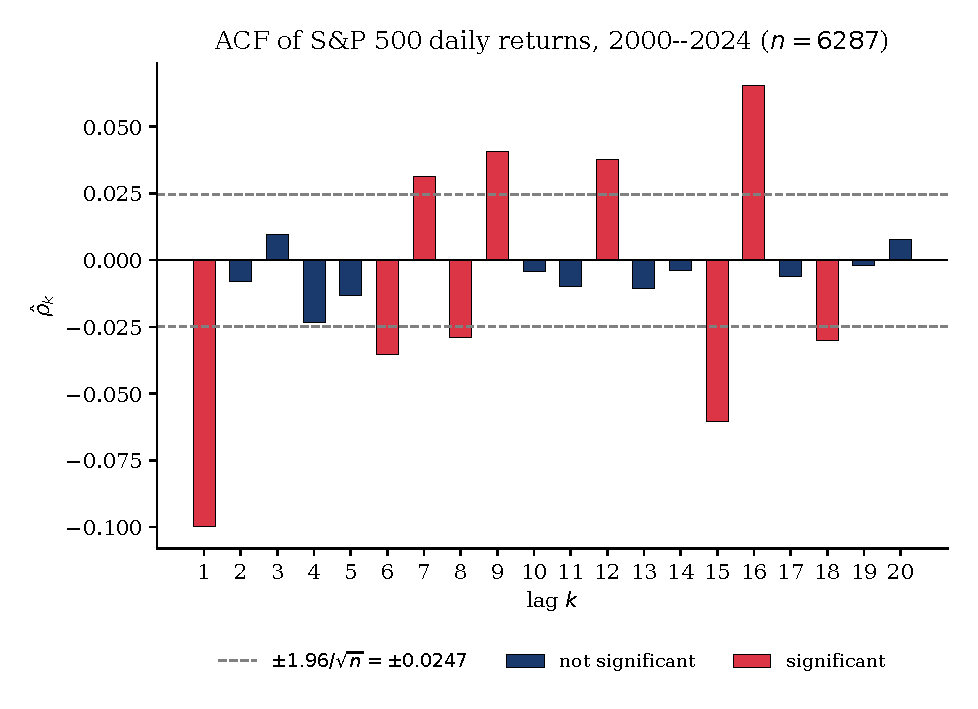
\includegraphics[width=\linewidth]{sfm_ch4_acf_sp500.pdf}
\end{column}
\begin{column}{0.37\textwidth}
\begin{itemize}\setlength{\itemsep}{0pt}
    \item Date: yfinance \texttt{\^{}GSPC}
    \begin{itemize}\setlength{\itemsep}{0pt}
        \item $n = 6.287$ observații zilnice
        \item Banda: $\pm 1{,}96/\sqrt{n} \approx \pm 0{,}025$
    \end{itemize}
    \item Observații
    \begin{itemize}\setlength{\itemsep}{0pt}
        \item Toate $|\hat\rho_k| < 0{,}025$
        \item Pattern compatibil cu EMH slabă
    \end{itemize}
    \item Contrast
    \begin{itemize}\setlength{\itemsep}{0pt}
        \item $r_t^2$ puternic autocorelate (GARCH)
        \item Dependență neliniară, nu liniară
    \end{itemize}
\end{itemize}
\end{column}
\end{columns}
\end{cminipage}
\vspace{0.05cm}
\quantlet{SFM\_ch4\_acf\_sp500}{https://colab.research.google.com/github/QuantLet/Stat_fin_markets/blob/master/Ch_04/SFM_ch4_acf_sp500/SFM_ch4_acf_sp500.ipynb}
\end{frame}

%=============================================================================
% PARTEA III: VARIANCE RATIO
%=============================================================================
\section{Partea III: Variance Ratio multi-piață}

\begin{frame}[shrink=15]{Testul variance ratio (VR test)}
\begin{cminipage}{0.95\textwidth}
\begin{block}{Formula și interpretare}
\begin{itemize}\setlength{\itemsep}{0pt}
    \item $VR(q) = \dfrac{\Var(r_t + \cdots + r_{t+q-1})}{q \cdot \Var(r_t)} = 1 + 2\sum_{k=1}^{q-1}\!\!\left(1 - \tfrac{k}{q}\right)\rho_k$
    \item Sub random walk: $VR(q) = 1$
    \item $VR > 1 \Rightarrow$ momentum (autocorelație pozitivă)
    \item $VR < 1 \Rightarrow$ mean reversion (autocorelație negativă)
\end{itemize}
\end{block}

\begin{exampleblock}{Statistica asimptotică (Lo \& MacKinlay, 1988)}
\begin{itemize}\setlength{\itemsep}{0pt}
    \item Sub homoscedasticitate: $Z(q) = \dfrac{VR(q) - 1}{\sqrt{2(q-1)/(T)}} \xrightarrow{d} \mathcal{N}(0, 1)$
    \item Sub heteroscedasticitate: ajustare robustă cu $\phi^*(k)$
    \item Decizie: $|Z| > 1{,}96 \Rightarrow$ respingem RW la 5\%
\end{itemize}
\end{exampleblock}
\end{cminipage}
\end{frame}

\begin{frame}[shrink=15]{Profilul VR(q) pe 3 piețe (2015--2024)}
\begin{cminipage}{0.95\textwidth}
\begin{columns}[T]
\begin{column}{0.6\textwidth}
\centering
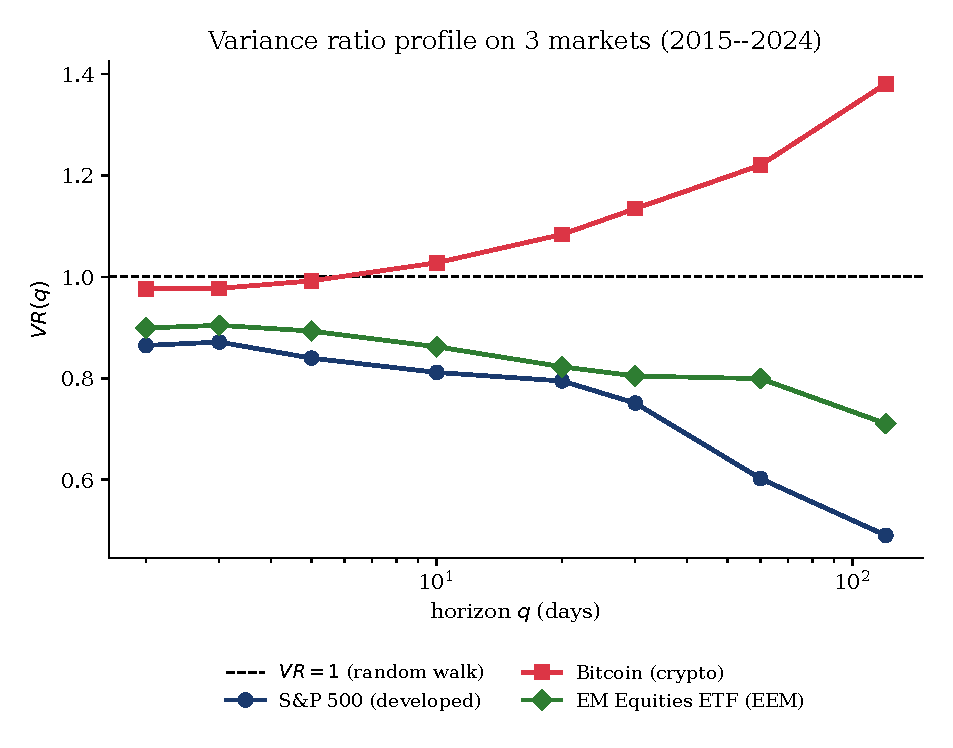
\includegraphics[width=\linewidth]{sfm_ch4_vr_profile.pdf}
\end{column}
\begin{column}{0.37\textwidth}
\begin{itemize}\setlength{\itemsep}{0pt}
    \item S\&P 500 (dezvoltată)
    \begin{itemize}\setlength{\itemsep}{0pt}
        \item $VR < 1$ pe orizonturi lungi
        \item Ușoară mean reversion
    \end{itemize}
    \item Bitcoin (crypto)
    \begin{itemize}\setlength{\itemsep}{0pt}
        \item $VR(120) = 1{,}38$
        \item Momentum puternic pe termen lung
    \end{itemize}
    \item EEM (emerging markets ETF)
    \begin{itemize}\setlength{\itemsep}{0pt}
        \item Pattern similar S\&P 500
        \item Dar volatilitate mai mare
    \end{itemize}
\end{itemize}
\end{column}
\end{columns}
\end{cminipage}
\vspace{0.05cm}
\quantlet{SFM\_ch4\_vr\_profile}{https://colab.research.google.com/github/QuantLet/Stat_fin_markets/blob/master/Ch_04/SFM_ch4_vr_profile/SFM_ch4_vr_profile.ipynb}
\end{frame}

%=============================================================================
% PARTEA IV: EVENT STUDY
%=============================================================================
\section{Partea IV: Event Study --- CAR}

\begin{frame}[shrink=15]{Metodologia event study}
\begin{cminipage}{0.95\textwidth}
\begin{block}{Etapele unui event study}
\begin{itemize}\setlength{\itemsep}{0pt}
    \item \textbf{Fereastra de estimare} $[-L, -M]$
    \begin{itemize}\setlength{\itemsep}{0pt}
        \item Estimăm modelul de piață: $r_{i,t} = \alpha + \beta r_{m,t} + \varepsilon_{i,t}$
    \end{itemize}
    \item \textbf{Fereastra de eveniment} $[-M+1, +T]$
    \begin{itemize}\setlength{\itemsep}{0pt}
        \item Calculăm AR (\textit{Abnormal Return}): $AR_{i,t} = r_{i,t} - (\hat\alpha + \hat\beta r_{m,t})$
    \end{itemize}
    \item \textbf{Cumulative AR}
    \begin{itemize}\setlength{\itemsep}{0pt}
        \item $CAR_i(t_1, t_2) = \sum_{t=t_1}^{t_2} AR_{i,t}$
        \item $\overline{CAR}(t_1, t_2) = \frac{1}{N}\sum_i CAR_i$
    \end{itemize}
    \item \textbf{Test de semnificație}
    \begin{itemize}\setlength{\itemsep}{0pt}
        \item $t = \overline{CAR}/(\hat\sigma_{CAR}/\sqrt{N}) \sim t_{\text{distribuție}}$
    \end{itemize}
\end{itemize}
\end{block}
\end{cminipage}
\end{frame}

\begin{frame}[shrink=15]{CAR: 3 scenarii + Apple}
\begin{cminipage}{0.95\textwidth}
\begin{columns}[T]
\begin{column}{0.6\textwidth}
\centering
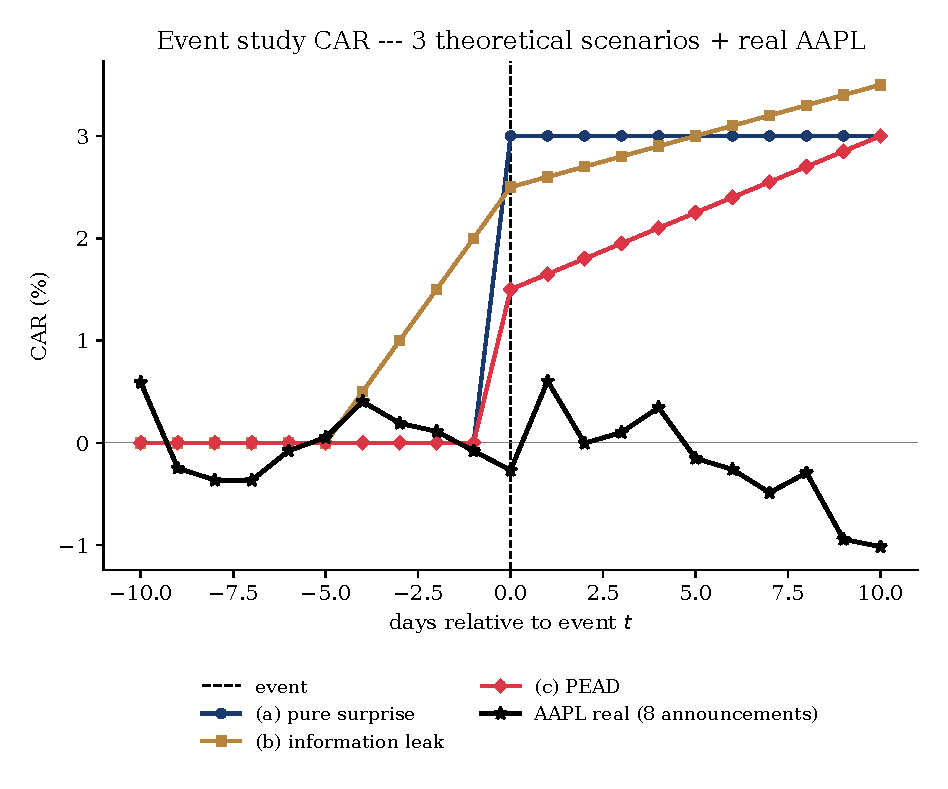
\includegraphics[width=\linewidth]{sfm_ch4_car_scenarios.pdf}
\end{column}
\begin{column}{0.37\textwidth}
\begin{itemize}\setlength{\itemsep}{0pt}
    \item (a) Surpriză pură
    \begin{itemize}\setlength{\itemsep}{0pt}
        \item Salt instant la $t = 0$
        \item Compatibil cu EMH semi-tare
    \end{itemize}
    \item (b) Leak (scurgere)
    \begin{itemize}\setlength{\itemsep}{0pt}
        \item Drift pre-eveniment
        \item Contrar EMH tare (insider)
    \end{itemize}
    \item (c) PEAD
    \begin{itemize}\setlength{\itemsep}{0pt}
        \item Drift post-eveniment
        \item Contrar EMH semi-tare
    \end{itemize}
    \item Apple (8 anunțuri, yfinance)
    \begin{itemize}\setlength{\itemsep}{0pt}
        \item Data: AAPL + SPY via yfinance
    \end{itemize}
\end{itemize}
\end{column}
\end{columns}
\end{cminipage}
\vspace{0.05cm}
\quantlet{SFM\_ch4\_car\_scenarios}{https://colab.research.google.com/github/QuantLet/Stat_fin_markets/blob/master/Ch_04/SFM_ch4_car_scenarios/SFM_ch4_car_scenarios.ipynb}
\end{frame}

%=============================================================================
% PARTEA V: HURST + AMH
%=============================================================================
\section{Partea V: Hurst + AMH}

\begin{frame}[shrink=15]{Exponentul Hurst și eficiența variabilă în timp}
\begin{cminipage}{0.95\textwidth}
\begin{columns}[T]
\begin{column}{0.58\textwidth}
\centering
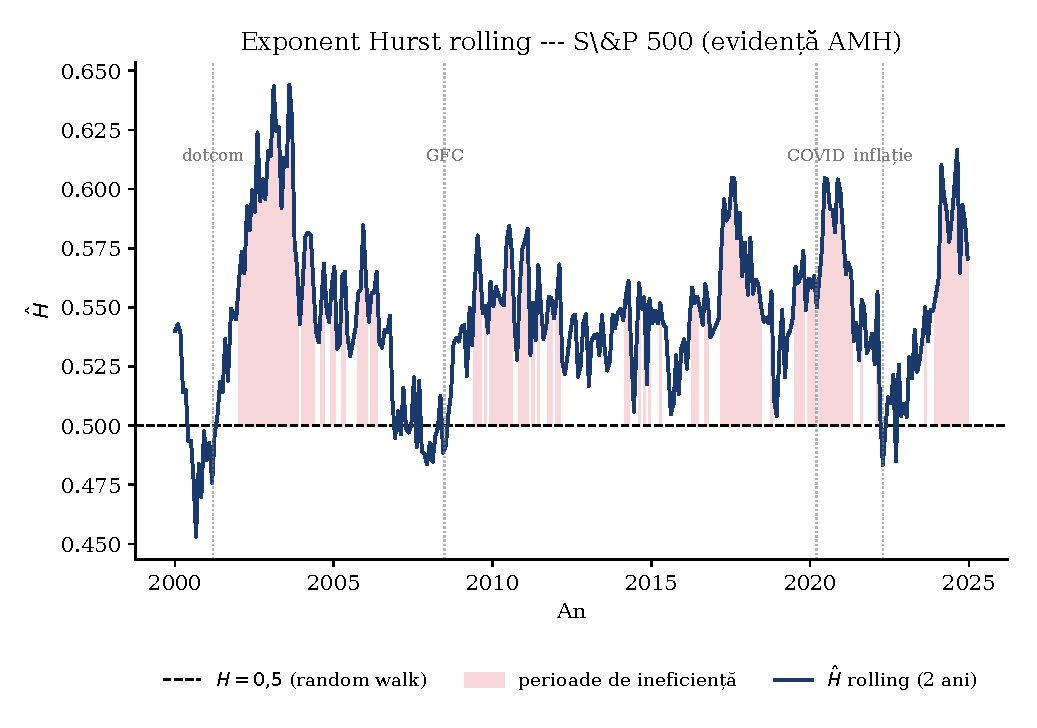
\includegraphics[width=\linewidth]{sfm_ch4_rolling_hurst.pdf}
\end{column}
\begin{column}{0.4\textwidth}
\begin{itemize}\setlength{\itemsep}{0pt}
    \item Exponentul Hurst (R/S)
    \begin{itemize}\setlength{\itemsep}{0pt}
        \item $H = 0{,}5$: random walk
        \item $H > 0{,}5$: memorie lungă (persistență)
        \item $H < 0{,}5$: anti-persistență (mean rev.)
    \end{itemize}
    \item Observații pe S\&P 500
    \begin{itemize}\setlength{\itemsep}{0pt}
        \item $\hat H$ oscilează $\sim 0{,}5$
        \item Crește $0{,}6$--$0{,}7$ în crize
    \end{itemize}
    \item AMH (Lo, 2004)
    \begin{itemize}\setlength{\itemsep}{0pt}
        \item Eficiența e dinamică
        \item Scade în crize, revine între
    \end{itemize}
\end{itemize}
\end{column}
\end{columns}
\end{cminipage}
\vspace{0.05cm}
\quantlet{SFM\_ch4\_rolling\_hurst}{https://colab.research.google.com/github/QuantLet/Stat_fin_markets/blob/master/Ch_04/SFM_ch4_rolling_hurst/SFM_ch4_rolling_hurst.ipynb}
\end{frame}

%=============================================================================
% PARTEA VI: MA crossover strategy
%=============================================================================
\section{Partea VI: Moving Average crossover}

\begin{frame}[shrink=15]{MA crossover: strategie clasică de trading}
\begin{cminipage}{0.95\textwidth}
\begin{block}{Regula Brock--Lakonishok--LeBaron (1992)}
\begin{itemize}\setlength{\itemsep}{0pt}
    \item Medie mobilă (MA, \textit{Moving Average}): $\text{MA}_t(k) = \frac{1}{k}\sum P_{t-i}$
    \item Cumpără când MA(50) $>$ MA(200) (Golden Cross)
    \item Vinde când MA(50) $<$ MA(200) (Death Cross)
    \item Ideea: exploatarea momentum-ului pe termen lung
\end{itemize}
\end{block}

\begin{alertblock}{Concluzie empirică}
\begin{itemize}\setlength{\itemsep}{0pt}
    \item Profitabilă pe date \textbf{pre-1990}
    \begin{itemize}\setlength{\itemsep}{0pt}
        \item BLL (1992) raportează excess return $\sim 3\%$/an
    \end{itemize}
    \item Dispare \textbf{post-1990}
    \begin{itemize}\setlength{\itemsep}{0pt}
        \item Piața se adaptează (consistent cu AMH)
        \item Costurile de tranzacție elimină profitul rămas
    \end{itemize}
\end{itemize}
\end{alertblock}
\end{cminipage}
\end{frame}

\begin{frame}[shrink=15]{Exemplu: MA(50)/MA(200) pe S\&P 500 (2010--2024)}
\begin{cminipage}{0.95\textwidth}
\centering
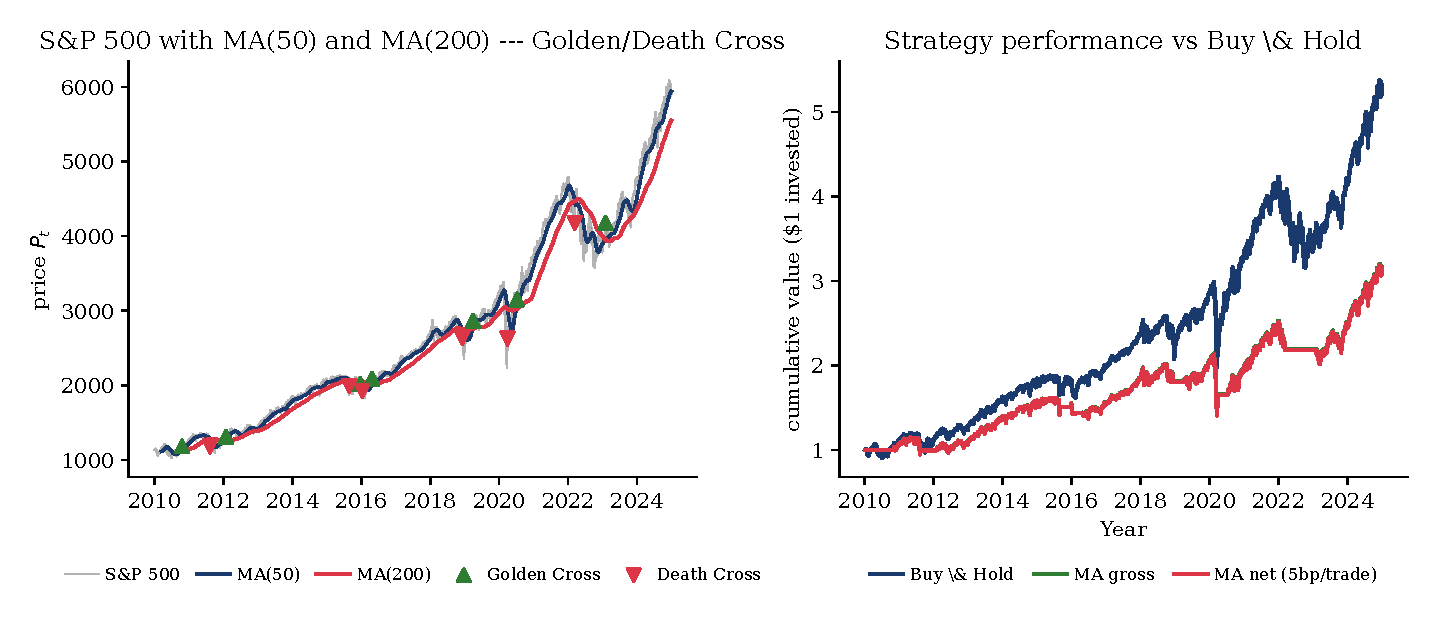
\includegraphics[width=\linewidth]{sfm_ch4_ma_crossover.pdf}
\end{cminipage}
\vspace{0.05cm}
\quantlet{SFM\_ch4\_ma\_crossover}{https://colab.research.google.com/github/QuantLet/Stat_fin_markets/blob/master/Ch_04/SFM_ch4_ma_crossover/SFM_ch4_ma_crossover.ipynb}
\end{frame}

\begin{frame}[shrink=15]{MA crossover: rezultate 2010--2024}
\begin{cminipage}{0.95\textwidth}
\begin{block}{Backtest pe 15 ani, S\&P 500, cu și fără costuri}
\begin{itemize}\setlength{\itemsep}{0pt}
    \item Buy \& Hold
    \begin{itemize}\setlength{\itemsep}{0pt}
        \item CAGR $= 11{,}65\%$; $\hat\sigma = 17{,}28\%$; Sharpe $= 0{,}56$
    \end{itemize}
    \item MA crossover \textbf{brut}
    \begin{itemize}\setlength{\itemsep}{0pt}
        \item CAGR $= 7{,}86\%$; $\hat\sigma = 13{,}73\%$; Sharpe $= 0{,}43$
        \item 13 tranzacții în 15 ani; $\sim 85\%$ timp în piață
    \end{itemize}
    \item MA crossover \textbf{net} (0{,}05\%/tranzacție)
    \begin{itemize}\setlength{\itemsep}{0pt}
        \item CAGR $= 7{,}81\%$; Sharpe $= 0{,}42$
    \end{itemize}
\end{itemize}
\end{block}

\begin{alertblock}{Verdict}
\begin{itemize}\setlength{\itemsep}{0pt}
    \item MA reduce $\sigma$ de la $17{,}3\%$ la $13{,}7\%$
    \item Dar pierde $\sim 3{,}8$pp de randament
    \item Sharpe B\&H ($0{,}56$) $>$ Sharpe MA ($0{,}42$)
    \item MA \textbf{nu} adaugă valoare ajustată la risc
    \item Consistent cu EMH slabă post-1990
\end{itemize}
\end{alertblock}
\end{cminipage}
\end{frame}

%=============================================================================
% PARTEA VII: SPIVA + ANOMALII
%=============================================================================
\section{Partea VII: Evidența SPIVA + bule}

\begin{frame}[shrink=15]{SPIVA: Active vs Passive (SPIVA Scorecard, 2024)}
\begin{cminipage}{0.95\textwidth}
\begin{columns}[T]
\begin{column}{0.58\textwidth}
\centering
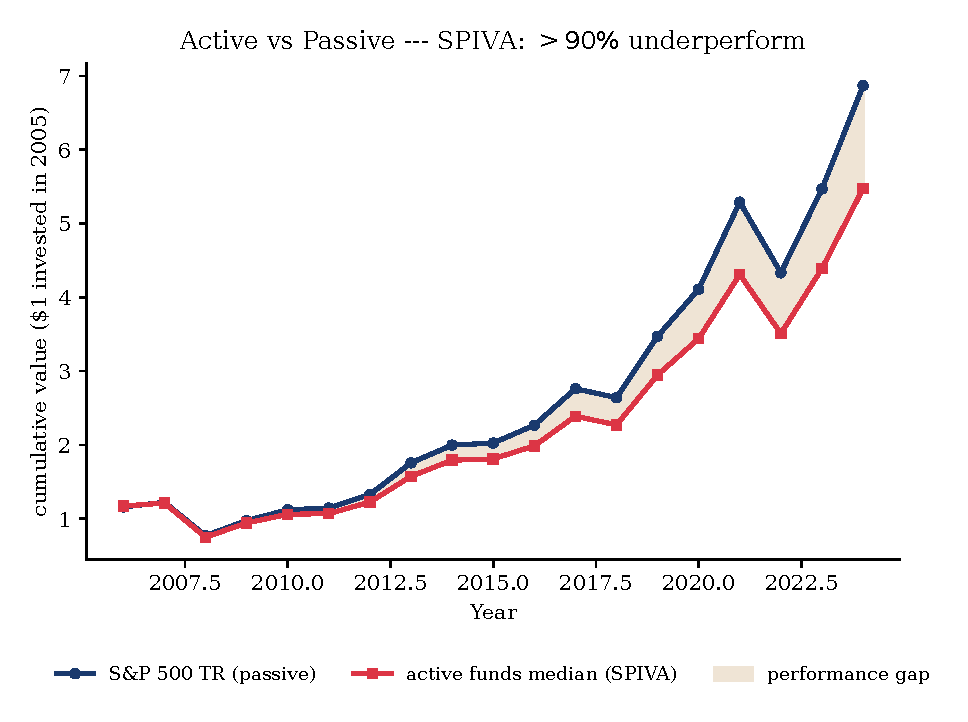
\includegraphics[width=\linewidth]{sfm_ch4_active_passive.pdf}
\end{column}
\begin{column}{0.4\textwidth}
\begin{itemize}\setlength{\itemsep}{0pt}
    \item Fapta empirică dominantă
    \begin{itemize}\setlength{\itemsep}{0pt}
        \item $> 90\%$ din fondurile active subperformează
        \item Gap-ul cumulativ în favoarea indicelui pasiv
    \end{itemize}
    \item Cauze
    \begin{itemize}\setlength{\itemsep}{0pt}
        \item Comisioane $\sim 1\%$/an
        \item Cost tranzacționare și slippage
        \item Competiție între manageri informați
    \end{itemize}
    \item Consecință
    \begin{itemize}\setlength{\itemsep}{0pt}
        \item Fondurile index pasive dominante
        \item Argument puternic pentru EMH
    \end{itemize}
\end{itemize}
\end{column}
\end{columns}
\end{cminipage}
\vspace{0.05cm}
\quantlet{SFM\_ch4\_active\_passive}{https://colab.research.google.com/github/QuantLet/Stat_fin_markets/blob/master/Ch_04/SFM_ch4_active_passive/SFM_ch4_active_passive.ipynb}
\end{frame}

\begin{frame}[shrink=15]{Bule și prăbușiri --- pattern-uri comparative}
\begin{cminipage}{0.95\textwidth}
\begin{columns}[T]
\begin{column}{0.58\textwidth}
\centering
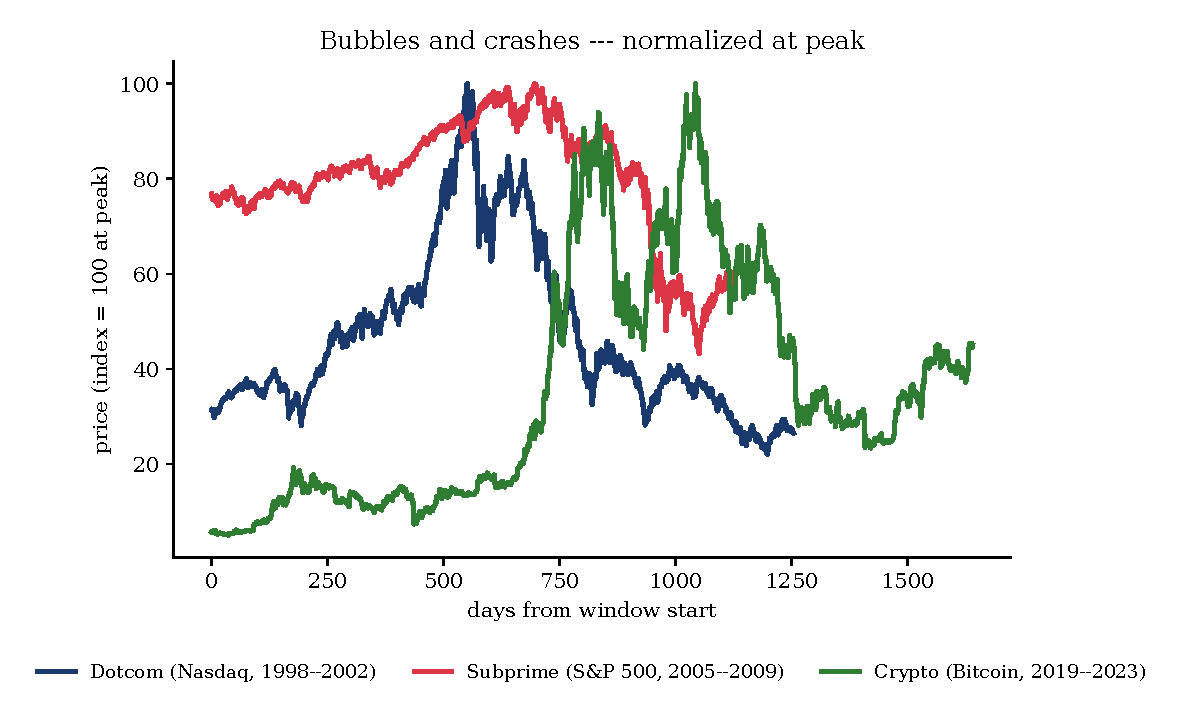
\includegraphics[width=\linewidth]{sfm_ch4_bubbles.pdf}
\end{column}
\begin{column}{0.4\textwidth}
\begin{itemize}\setlength{\itemsep}{0pt}
    \item Pattern universal
    \begin{itemize}\setlength{\itemsep}{0pt}
        \item Creștere exponențială înainte de vârf
        \item Vârf abrupt, urmat de cădere
        \item Asimetrie: urcăm lent, cădem rapid
    \end{itemize}
    \item Trei exemple
    \begin{itemize}\setlength{\itemsep}{0pt}
        \item Dotcom (Nasdaq, 2000)
        \item Subprime (S\&P 500, 2007--2008)
        \item Crypto (Bitcoin, 2021)
    \end{itemize}
    \item Lecția pentru EMH
    \begin{itemize}\setlength{\itemsep}{0pt}
        \item Bulele persistă în ciuda testelor
        \item Arbitrajul este costisitor și riscant
    \end{itemize}
\end{itemize}
\end{column}
\end{columns}
\end{cminipage}
\vspace{0.05cm}
\quantlet{SFM\_ch4\_bubbles}{https://colab.research.google.com/github/QuantLet/Stat_fin_markets/blob/master/Ch_04/SFM_ch4_bubbles/SFM_ch4_bubbles.ipynb}
\end{frame}

%=============================================================================
% PARTEA VIII: EXERCITII
%=============================================================================
\section{Partea VIII: Exerciții}

\begin{frame}[shrink=15]{Exercițiul 1: Ljung--Box pe BVB}
\begin{cminipage}{0.95\textwidth}
\begin{block}{Enunț}
\begin{itemize}\setlength{\itemsep}{0pt}
    \item Pe $T = 250$ randamente zilnice BET se observă:
    \begin{itemize}\setlength{\itemsep}{0pt}
        \item $\hat\rho_1 = 0{,}12$; $\hat\rho_2 = 0{,}05$; $\hat\rho_3 = 0{,}03$
        \item $\hat\rho_4 = -0{,}02$; $\hat\rho_5 = 0{,}08$
    \end{itemize}
\end{itemize}
\end{block}

\begin{itemize}\setlength{\itemsep}{0pt}
    \item \textbf{Cerințe}
    \begin{itemize}\setlength{\itemsep}{0pt}
        \item Calculați $Q(5)$ folosind $Q(m) = T(T+2)\sum_{k=1}^{m}\frac{\hat\rho_k^2}{T-k}$
        \item Testați $H_0$ la $\alpha = 5\%$ cu $\chi^2_5(0{,}05) = 11{,}07$
        \item Interpretați economic vs EMH slabă
    \end{itemize}
\end{itemize}
\end{cminipage}
\end{frame}

\begin{frame}[shrink=15]{Exercițiul 1: Rezolvare}
\begin{cminipage}{0.95\textwidth}
\begin{exampleblock}{Rezolvare}
\begin{itemize}\setlength{\itemsep}{0pt}
    \item \textbf{Calculul $Q(5)$}
    \begin{itemize}\setlength{\itemsep}{0pt}
        \item $T(T+2) = 250 \cdot 252 = 63.000$
        \item Sumă: $\frac{0{,}12^2}{249} + \frac{0{,}05^2}{248} + \frac{0{,}03^2}{247} + \frac{0{,}02^2}{246} + \frac{0{,}08^2}{245}$
        \item $= 5{,}78 \cdot 10^{-5} + 1{,}01 \cdot 10^{-5} + 3{,}64 \cdot 10^{-6} + 1{,}63 \cdot 10^{-6} + 2{,}61 \cdot 10^{-5}$
        \item Total $\approx 9{,}71 \cdot 10^{-5}$
        \item $Q(5) = 63.000 \cdot 9{,}71 \cdot 10^{-5} \approx \mathbf{6{,}12}$
    \end{itemize}
    \item \textbf{Decizia}
    \begin{itemize}\setlength{\itemsep}{0pt}
        \item $Q(5) = 6{,}12 < 11{,}07 \Rightarrow$ nu respingem $H_0$ la 5\%
    \end{itemize}
    \item \textbf{Interpretare}
    \begin{itemize}\setlength{\itemsep}{0pt}
        \item La nivel 5\%, BET este compatibil cu EMH slabă
        \item Notă: $\hat\rho_1 = 0{,}12$ ar putea fi relevant pe eșantion mai mare
    \end{itemize}
\end{itemize}
\end{exampleblock}
\end{cminipage}
\end{frame}

\begin{frame}[shrink=15]{Exercițiul 2: Variance Ratio}
\begin{cminipage}{0.95\textwidth}
\begin{block}{Enunț}
\begin{itemize}\setlength{\itemsep}{0pt}
    \item Pe un activ se observă:
    \begin{itemize}\setlength{\itemsep}{0pt}
        \item $\hat\sigma^2_1 = 0{,}0001$ (varianța randamentelor zilnice)
        \item $\hat\sigma^2_5 = 0{,}000575$ (varianța randamentelor cumulate pe 5 zile)
        \item $T = 1.000$ observații zilnice
    \end{itemize}
\end{itemize}
\end{block}

\begin{itemize}\setlength{\itemsep}{0pt}
    \item \textbf{Cerințe}
    \begin{itemize}\setlength{\itemsep}{0pt}
        \item Calculați $VR(5) = \sigma^2_5 / (5 \cdot \sigma^2_1)$
        \item Calculați statistica $Z = (VR - 1)/\sqrt{2(q-1)/T}$
        \item Testați RW la $\alpha = 5\%$ ($z_{0{,}025} = 1{,}96$)
        \item Interpretați (momentum sau mean reversion)
    \end{itemize}
\end{itemize}
\end{cminipage}
\end{frame}

\begin{frame}[shrink=15]{Exercițiul 2: Rezolvare}
\begin{cminipage}{0.95\textwidth}
\begin{exampleblock}{Rezolvare}
\begin{itemize}\setlength{\itemsep}{0pt}
    \item \textbf{Calculul VR(5)}
    \begin{itemize}\setlength{\itemsep}{0pt}
        \item $VR(5) = 0{,}000575/(5 \cdot 0{,}0001) = 0{,}000575/0{,}0005 = \mathbf{1{,}15}$
    \end{itemize}
    \item \textbf{Statistica $Z$}
    \begin{itemize}\setlength{\itemsep}{0pt}
        \item $Z = (1{,}15 - 1)/\sqrt{2 \cdot 4/1000} = 0{,}15/\sqrt{0{,}008} = 0{,}15/0{,}0894$
        \item $Z \approx \mathbf{1{,}68}$
    \end{itemize}
    \item \textbf{Decizia}
    \begin{itemize}\setlength{\itemsep}{0pt}
        \item $|Z| = 1{,}68 < 1{,}96 \Rightarrow$ nu respingem RW la 5\%
        \item Marginal: $p \approx 0{,}09$ (semnificativ la 10\%)
    \end{itemize}
    \item \textbf{Interpretare}
    \begin{itemize}\setlength{\itemsep}{0pt}
        \item $VR > 1 \Rightarrow$ tendință de momentum
        \item Statistic nesemnificativ la 5\%
        \item Economic: pe termen de 5 zile, randamentele au ușoară persistență
    \end{itemize}
\end{itemize}
\end{exampleblock}
\end{cminipage}
\end{frame}

\begin{frame}[shrink=15]{Exercițiul 3: Event Study CAR}
\begin{cminipage}{0.95\textwidth}
\begin{block}{Enunț}
\begin{itemize}\setlength{\itemsep}{0pt}
    \item Anunț neașteptat la $t = 0$; fereastra $[-2, +3]$:
    \begin{itemize}\setlength{\itemsep}{0pt}
        \item $AR$ (\%): $-0{,}2$; $0{,}1$; $\mathbf{2{,}8}$; $0{,}6$; $-0{,}1$; $0{,}2$ (pentru $t = -2, \ldots, +3$)
        \item Deviația std.\ pe fereastra de estimare: $\hat\sigma_{AR} = 1{,}3\%$
    \end{itemize}
\end{itemize}
\end{block}

\begin{itemize}\setlength{\itemsep}{0pt}
    \item \textbf{Cerințe}
    \begin{itemize}\setlength{\itemsep}{0pt}
        \item Calculați CAR$[-2, +3]$
        \item Testați $H_0: CAR = 0$ cu $t = CAR/(\hat\sigma_{AR}\sqrt{L})$
        \item Este evenimentul surpriză pură, leak sau PEAD?
        \item Concluzia pentru EMH semi-tare
    \end{itemize}
\end{itemize}
\end{cminipage}
\end{frame}

\begin{frame}[shrink=15]{Exercițiul 3: Rezolvare}
\begin{cminipage}{0.95\textwidth}
\begin{exampleblock}{Rezolvare}
\begin{itemize}\setlength{\itemsep}{0pt}
    \item \textbf{CAR}
    \begin{itemize}\setlength{\itemsep}{0pt}
        \item $CAR[-2, +3] = -0{,}2 + 0{,}1 + 2{,}8 + 0{,}6 - 0{,}1 + 0{,}2 = \mathbf{3{,}4\%}$
    \end{itemize}
    \item \textbf{Testul $t$}
    \begin{itemize}\setlength{\itemsep}{0pt}
        \item $L = 6$; $t = 3{,}4/(1{,}3 \cdot \sqrt{6}) = 3{,}4/3{,}18 \approx \mathbf{1{,}07}$
        \item $|t| < 1{,}96 \Rightarrow$ nu respingem pe eveniment individual
        \item Agregat pe $N$ evenimente crește puterea testului
    \end{itemize}
    \item \textbf{Diagnostic}
    \begin{itemize}\setlength{\itemsep}{0pt}
        \item $AR_{-2}, AR_{-1}$ foarte mici $\Rightarrow$ \textbf{nu există leak}
        \item Salt $+2{,}8\%$ la $t=0$, $+0{,}6\%$ la $t=+1$ $\Rightarrow$ \textbf{surpriză pură}
        \item Ajustare rapidă (1--2 zile)
    \end{itemize}
    \item \textbf{Concluzie EMH semi-tare}
    \begin{itemize}\setlength{\itemsep}{0pt}
        \item Ajustare rapidă la info publică $\Rightarrow$ compatibil cu EMH semi-tare
    \end{itemize}
\end{itemize}
\end{exampleblock}
\end{cminipage}
\end{frame}

%=============================================================================
% A/F
%=============================================================================
\section{Test rapid: Adevărat/Fals}

\begin{frame}[shrink=15]{Adevărat sau Fals? (1/2)}
\begin{cminipage}{0.95\textwidth}
\begin{columns}[T]
\begin{column}{0.48\textwidth}
\begin{itemize}\setlength{\itemsep}{1pt}
    \item ,,EMH implică randamente zero.''
    \begin{itemize}\setlength{\itemsep}{0pt}
        \item[] \textcolor{Crimson}{\textbf{Fals.}} EMH cere doar că \emph{randamentele neașteptate} sunt zero în medie. Investitorii câștigă prima de risc.
    \end{itemize}
    \item ,,EMH $\Leftrightarrow$ random walk.''
    \begin{itemize}\setlength{\itemsep}{0pt}
        \item[] \textcolor{Crimson}{\textbf{Fals.}} EMH implică martingal pt.\ prețuri ajustate la risc, nu incremente iid. GARCH compatibil.
    \end{itemize}
    \item ,,$VR > 1$ indică mean reversion.''
    \begin{itemize}\setlength{\itemsep}{0pt}
        \item[] \textcolor{Crimson}{\textbf{Fals.}} $VR > 1$ = momentum; $VR < 1$ = mean reversion.
    \end{itemize}
\end{itemize}
\end{column}
\begin{column}{0.48\textwidth}
\begin{itemize}\setlength{\itemsep}{1pt}
    \item ,,ACF randamente $\approx 0 \Rightarrow$ EMH slabă.''
    \begin{itemize}\setlength{\itemsep}{0pt}
        \item[] \textcolor{Forest}{\textbf{Adevărat.}} ACF zero $\Rightarrow$ impredictibilitate liniară, compatibil EMH slabă.
    \end{itemize}
    \item ,,PEAD contrazice EMH semi-tare.''
    \begin{itemize}\setlength{\itemsep}{0pt}
        \item[] \textcolor{Forest}{\textbf{Adevărat.}} Drift predictibil post-anunț $\Rightarrow$ piața nu încorporează rapid info publică.
    \end{itemize}
    \item ,,Insider trading profitabil $\Rightarrow$ respinge EMH tare.''
    \begin{itemize}\setlength{\itemsep}{0pt}
        \item[] \textcolor{Forest}{\textbf{Adevărat.}} Forma tare cere că nici info privată nu generează alpha.
    \end{itemize}
\end{itemize}
\end{column}
\end{columns}
\end{cminipage}
\end{frame}

\begin{frame}[shrink=15]{Adevărat sau Fals? (2/2)}
\begin{cminipage}{0.95\textwidth}
\begin{columns}[T]
\begin{column}{0.48\textwidth}
\begin{itemize}\setlength{\itemsep}{1pt}
    \item ,,$H = 0{,}5$ este condiție suficientă pentru EMH slabă.''
    \begin{itemize}\setlength{\itemsep}{0pt}
        \item[] \textcolor{Crimson}{\textbf{Fals.}} Necesară dar nu suficientă. Dependențe neliniare posibile.
    \end{itemize}
    \item ,,AMH contrazice EMH.''
    \begin{itemize}\setlength{\itemsep}{0pt}
        \item[] \textcolor{Crimson}{\textbf{Fals.}} AMH este generalizare. EMH e caz special (eficiență constantă).
    \end{itemize}
    \item ,,$>90\%$ fonduri active subperformează indicele.''
    \begin{itemize}\setlength{\itemsep}{0pt}
        \item[] \textcolor{Forest}{\textbf{Adevărat.}} SPIVA Scorecard 2024 pe 15 ani.
    \end{itemize}
\end{itemize}
\end{column}
\begin{column}{0.48\textwidth}
\begin{itemize}\setlength{\itemsep}{1pt}
    \item ,,MA crossover generează alpha pe S\&P 500 post-1990.''
    \begin{itemize}\setlength{\itemsep}{0pt}
        \item[] \textcolor{Crimson}{\textbf{Fals.}} MA crossover subperformează B\&H post-1990 după costuri.
    \end{itemize}
    \item ,,Ljung--Box pe $r_t^2$ detectează clustering volatilitate.''
    \begin{itemize}\setlength{\itemsep}{0pt}
        \item[] \textcolor{Forest}{\textbf{Adevărat.}} Standard în literatură (efect ARCH).
    \end{itemize}
    \item ,,Bulele contrazic EMH pe piețele dezvoltate.''
    \begin{itemize}\setlength{\itemsep}{0pt}
        \item[] \textcolor{Amber}{\textbf{Parțial.}} \emph{Ex post} evident; \emph{ex ante} greu de exploatat (arbitraj costisitor).
    \end{itemize}
\end{itemize}
\end{column}
\end{columns}
\end{cminipage}
\end{frame}

%=============================================================================
% CONCLUZII
%=============================================================================
\section{Concluzii}

\begin{frame}[shrink=15]{Concluzii și mesaje cheie}
\begin{cminipage}{0.95\textwidth}
\begin{block}{Ce am învățat}
\begin{itemize}\setlength{\itemsep}{0pt}
    \item \textbf{Formele EMH} (Fama, 1970)
    \begin{itemize}\setlength{\itemsep}{0pt}
        \item Slabă / Semi-tare / Tare --- ierarhie incluzivă
    \end{itemize}
    \item \textbf{Teste} pe date financiare
    \begin{itemize}\setlength{\itemsep}{0pt}
        \item ACF + Ljung--Box (S\&P 500: compatibil EMH slabă)
        \item Variance ratio (multi-piață: BTC momentum, SP mean rev.)
        \item Event study CAR (Apple: surpriză pură $\Rightarrow$ EMH semi-tare ok)
        \item Hurst rolling (AMH: eficiența variază cu crizele)
    \end{itemize}
    \item \textbf{Strategii testate}
    \begin{itemize}\setlength{\itemsep}{0pt}
        \item MA crossover: subperformează după costuri
        \item Active vs Passive: $>90\%$ subperformează
    \end{itemize}
\end{itemize}
\end{block}

\begin{alertblock}{Regula de aur}
\begin{itemize}\setlength{\itemsep}{0pt}
    \item Piețele sunt ,,eficient ineficiente'' (Pedersen, 2015)
    \begin{itemize}\setlength{\itemsep}{0pt}
        \item Suficient de eficiente încât majoritatea nu le pot bate
        \item Cu suficiente fricțiuni pentru traderi sofisticați
    \end{itemize}
\end{itemize}
\end{alertblock}
\end{cminipage}
\end{frame}

\begin{frame}[shrink=15]{Quantlets disponibile pe Colab}
\begin{cminipage}{0.95\textwidth}
\begin{block}{Toate notebook-urile pot fi executate direct pe Google Colab}
\begin{itemize}\setlength{\itemsep}{0pt}
    \item \textbf{Teste de eficiență}
    \begin{itemize}\setlength{\itemsep}{0pt}
        \item \href{https://colab.research.google.com/github/QuantLet/Stat_fin_markets/blob/master/Ch_04/SFM_ch4_acf_sp500/SFM_ch4_acf_sp500.ipynb}{SFM\_ch4\_acf\_sp500}: ACF S\&P 500 2000--2024
        \item \href{https://colab.research.google.com/github/QuantLet/Stat_fin_markets/blob/master/Ch_04/SFM_ch4_vr_profile/SFM_ch4_vr_profile.ipynb}{SFM\_ch4\_vr\_profile}: VR multi-piață
        \item \href{https://colab.research.google.com/github/QuantLet/Stat_fin_markets/blob/master/Ch_04/SFM_ch4_rolling_hurst/SFM_ch4_rolling_hurst.ipynb}{SFM\_ch4\_rolling\_hurst}: Hurst rolling S\&P 500
    \end{itemize}
    \item \textbf{Event study \& strategii}
    \begin{itemize}\setlength{\itemsep}{0pt}
        \item \href{https://colab.research.google.com/github/QuantLet/Stat_fin_markets/blob/master/Ch_04/SFM_ch4_car_scenarios/SFM_ch4_car_scenarios.ipynb}{SFM\_ch4\_car\_scenarios}: CAR AAPL + 3 scenarii
        \item \href{https://colab.research.google.com/github/QuantLet/Stat_fin_markets/blob/master/Ch_04/SFM_ch4_ma_crossover/SFM_ch4_ma_crossover.ipynb}{SFM\_ch4\_ma\_crossover}: MA(50)/MA(200) S\&P 500
    \end{itemize}
    \item \textbf{Comparații și bule}
    \begin{itemize}\setlength{\itemsep}{0pt}
        \item \href{https://colab.research.google.com/github/QuantLet/Stat_fin_markets/blob/master/Ch_04/SFM_ch4_active_passive/SFM_ch4_active_passive.ipynb}{SFM\_ch4\_active\_passive}: SPIVA
        \item \href{https://colab.research.google.com/github/QuantLet/Stat_fin_markets/blob/master/Ch_04/SFM_ch4_bubbles/SFM_ch4_bubbles.ipynb}{SFM\_ch4\_bubbles}: Dotcom/Subprime/Crypto
        \item \href{https://colab.research.google.com/github/QuantLet/Stat_fin_markets/blob/master/Ch_04/SFM_ch4_rw_sim/SFM_ch4_rw_sim.ipynb}{SFM\_ch4\_rw\_sim}: Random walk vs S\&P 500
    \end{itemize}
\end{itemize}
\end{block}
\end{cminipage}
\end{frame}

\begin{frame}[shrink=15]{Bibliografie}
\begin{cminipage}{0.95\textwidth}
\begin{itemize}\setlength{\itemsep}{0pt}
    \item \textbf{Clasic}
    \begin{itemize}\setlength{\itemsep}{0pt}
        \item Fama (1970). Efficient Capital Markets. \textit{Journal of Finance}, 25(2).
        \item Fama (1991). Efficient Capital Markets: II. \textit{Journal of Finance}, 46(5).
        \item Lo \& MacKinlay (1988). Stock Market Prices Do Not Follow Random Walks. \textit{RFS}, 1(1).
    \end{itemize}
    \item \textbf{Anomalii și behavioral}
    \begin{itemize}\setlength{\itemsep}{0pt}
        \item Ball \& Brown (1968). \textit{Journal of Accounting Research} (PEAD)
        \item Shiller (1981). Excess Volatility. \textit{AER}, 71(3).
        \item De Bondt \& Thaler (1985). Overreaction. \textit{Journal of Finance}, 40(3).
    \end{itemize}
    \item \textbf{Modern}
    \begin{itemize}\setlength{\itemsep}{0pt}
        \item Lo (2004). Adaptive Markets Hypothesis. \textit{JPM}, 30(5).
        \item Pedersen (2015). \textit{Efficiently Inefficient}. Princeton.
        \item McLean \& Pontiff (2016). Does Publication Predict Stock Returns? \textit{JoF}.
    \end{itemize}
\end{itemize}
\end{cminipage}
\end{frame}

\end{document}
